% !TEX spellcheck = en_US



% ~~~~~~~~~~~~~~~~~~~~~~~~~~~~~~~~~~~~~~~ V
% (NC) 2026 Haluk Bingol
% github.com/halukbingol/LaTeX-Templates
%
% Licensees may copy, distribute, display, and perform the work and make derivative works 
% and remixes based on it only for non-commercial purposes. 
% ~~~~~~~~~~~~~~~~~~~~~~~~~~~~~~~~~~~~~~~ A




% =====================================================================
%  Regular Expressions in Java -- Concepts: Patterns, Building Blocks, Engines and Limits
%  ---------------------------------------------------------------------
%  Built on hblib/Template/hblibTemplate.tex with the libraries in ../../hblib/.
%  Programs and their real outputs are in codeoutput/:
%     codeoutput/<Name>.java  a program (classes without main() are only compiled)
%     codeoutput/<Name>.sh    a terminal session, run in a copy of codeoutput/<Name>/
%     codeoutput/<Name>.txt   what it printed, made by:  bash run_examples.sh
% =====================================================================

\documentclass[aspectratio=169,10pt,compress]{beamer}

% ~~~~~~~~~~~~~~~~~~~~~~~~~~~~~~~~~~~~~~~~~~~~~~~~~~~~~~~~~~~~~~~~~ V hblib
	\usepackage{../../hblib/hblibPresentation} % lib presentation: theme, i/N, \hSection, algorithm2e, ...
	\usepackage{../../hblib/hblibCodeoutput} % lib code + output: \lstcode, \lstterminal, ...
	\usepackage{../../hblib/hblibDatastructures} % lib data structures: \hString, \hStack, \hQueue
% ~~~~~~~~~~~~~~~~~~~~~~~~~~~~~~~~~~~~~~~~~~~~~~~~~~~~~~~~~~~~~~~~~ A hblib


% theme, i/N, fonts (T1, lmodern), booktabs, xcolor, array (L{width} columns), listings, tikz,
% algorithm2e (\small captions, \Fn) and the color gitred come from the hblib libraries




% +++++++++++++++++++++++++++++++++++++++ V specific
\DontPrintSemicolon % in algorithms
\newcommand{\win}{\textbf{Windows}}
\newcommand{\mac}{\textbf{macOS}}
\usetikzlibrary{automata,positioning}
% +++++++++++++++++++++++++++++++++++++++ A specific

% ---------------------------------------------------------------------
\title{Regular Expressions in Java}
\subtitle{Concepts: Patterns, Building Blocks, Engines and Limits}
\author[Bingol]{Haluk O. Bingol}

\institute[FCIS]{
    Faculty of Computer and Information Sciences\\
    Yeditepe University
}
\date{
	{\tiny \hbTimeStamp}
}

\begin{document}




% ~~~~~~~~~~~~~~~~~~~~~~~~~~~~~~~~~~~~~~ V frm
\begin{frame}[t,fragile]
  \titlepage
\end{frame}
% ~~~~~~~~~~~~~~~~~~~~~~~~~~~~~~~~~~~~~~ A frm




% ~~~~~~~~~~~~~~~~~~~~~~~~~~~~~~~~~~~~~~ V frm
\begin{frame}[t,fragile] \frametitle{Outline}
  \begin{columns}[T]
    \begin{column}{0.48\textwidth}
      \tableofcontents[sections={1-4}, hideallsubsections]
    \end{column}
    \begin{column}{0.48\textwidth}
      \tableofcontents[sections={5-8}, hideallsubsections]
    \end{column}
  \end{columns}
\end{frame}
% ~~~~~~~~~~~~~~~~~~~~~~~~~~~~~~~~~~~~~~ A frm

% ~~~~~~~~~~~~~~~~~~~~~~~~~~~~~~~~~~~~~~ V
\hSection[Idea]{The Idea}
% ~~~~~~~~~~~~~~~~~~~~~~~~~~~~~~~~~~~~~~ A




% ~~~~~~~~~~~~~~~~~~~~~~~~~~~~~~~~~~~~~~ V frm
\begin{frame}[t,fragile] \frametitle{A pattern describes a set of strings}
  \begin{columns}[T]
    \begin{column}{0.5\textwidth}
      \begin{itemize}\small
        \item A \textbf{regular expression} (regex) is a small formula for text.
        \item It stands for a \emph{set} of strings: ``four digits'', ``a word with a capital first letter'', ``a Yeditepe student e-mail''.
        \item A string \textbf{matches} the regex if it is in the set.
        \item One line of regex replaces a loop with many \texttt{if}s.
      \end{itemize}
    \end{column}
    \begin{column}{0.46\textwidth}
      \begin{center}\small
      \begin{tabular}{@{}lll@{}}
        \toprule
        \textbf{regex}                       & \textbf{matches}  & \textbf{does not} \\
        \midrule
        \texttt{cat}                         & cat               & Cat, cats \\
        \texttt{c.t}                         & cat, cut, c9t     & ct, cart \\
        \texttt{ca*t}                        & ct, cat, caaat    & cut \\
        \texttt{[0-9]\{4\}}                  & 2026, 0042        & 202, 20a6 \\
        \texttt{cat|dog}                     & cat, dog          & cow \\
        \bottomrule
      \end{tabular}
      \end{center}
    \end{column}
  \end{columns}
\end{frame}
% ~~~~~~~~~~~~~~~~~~~~~~~~~~~~~~~~~~~~~~ A frm




% ~~~~~~~~~~~~~~~~~~~~~~~~~~~~~~~~~~~~~~ V frm
\begin{frame}[t,fragile] \frametitle{Four things we do with a regex}
  \begin{center}\small
  \begin{tabular}{@{}L{0.16\textwidth}L{0.38\textwidth}L{0.38\textwidth}@{}}
    \toprule
    \textbf{task}      & \textbf{question}                                  & \textbf{example} \\
    \midrule
    validate           & Is the whole text of this form?                    & a student number has 11 digits \\
    search             & Where does the form occur?                         & every date in a report \\
    extract            & What are the parts?                                & year, month, day of a date \\
    transform          & Replace or cut at the matches                      & \texttt{26.10.2026} $\to$ \texttt{2026-10-26}; split a CSV line \\
    \bottomrule
  \end{tabular}
  \end{center}
  \begin{itemize}\small
    \item Everywhere: Java, Python, JavaScript, databases, \texttt{grep}, text editors and IDEs (Find with ``Regular expressions'').
    \item The core syntax is shared; each tool adds its own extras.
  \end{itemize}
\end{frame}
% ~~~~~~~~~~~~~~~~~~~~~~~~~~~~~~~~~~~~~~ A frm

% ~~~~~~~~~~~~~~~~~~~~~~~~~~~~~~~~~~~~~~ V
\hSection[Blocks]{Building Blocks}
% ~~~~~~~~~~~~~~~~~~~~~~~~~~~~~~~~~~~~~~ A




% ~~~~~~~~~~~~~~~~~~~~~~~~~~~~~~~~~~~~~~ V frm
\begin{frame}[t,fragile] \frametitle{Characters and classes}
  \begin{center}\small
  \begin{tabular}{@{}L{0.2\textwidth}L{0.42\textwidth}L{0.3\textwidth}@{}}
    \toprule
    \textbf{regex}                                   & \textbf{meaning}                       & \textbf{example match} \\
    \midrule
    \texttt{a}                                       & the letter a itself (a \emph{literal}) & a \\
    \texttt{.}                                       & any one character (not a newline)      & a, 7, \% \\
    \texttt{[aeıioöuü]}                              & one of these                           & ö \\
    \texttt{[a-z]}, \texttt{[0-9]}                   & one in this range                      & k, 4 \\
    \texttt{[\textasciicircum 0-9]}                  & one \emph{not} in the set              & x \\
    \texttt{\textbackslash d}, \texttt{\textbackslash w}, \texttt{\textbackslash s} & digit, word character, white space & 5, \_, (space) \\
    \texttt{\textbackslash p\{L\}}                   & any letter, also Turkish               & ğ \\
    \texttt{\textbackslash .}, \texttt{\textbackslash *} & the character itself (\emph{escaped}) & ., * \\
    \bottomrule
  \end{tabular}
  \end{center}
  \small Special characters: \texttt{. [ ] ( ) \{ \} * + ? \textasciicircum{} \$ | \textbackslash}; a \texttt{\textbackslash} before one makes it ordinary.
\end{frame}
% ~~~~~~~~~~~~~~~~~~~~~~~~~~~~~~~~~~~~~~ A frm




% ~~~~~~~~~~~~~~~~~~~~~~~~~~~~~~~~~~~~~~ V frm
\begin{frame}[t,fragile] \frametitle{Repetition, position, grouping}
  \begin{columns}[T]
    \begin{column}{0.48\textwidth}
      \begin{center}\small
      \begin{tabular}{@{}ll@{}}
        \toprule
        \textbf{quantifier}      & \textbf{how many times} \\
        \midrule
        \texttt{x?}              & 0 or 1 \\
        \texttt{x*}              & 0 or more \\
        \texttt{x+}              & 1 or more \\
        \texttt{x\{3\}}          & exactly 3 \\
        \texttt{x\{2,4\}}        & 2 to 4 \\
        \texttt{x\{2,\}}         & 2 or more \\
        \bottomrule
      \end{tabular}
      \end{center}
    \end{column}
    \begin{column}{0.48\textwidth}
      \begin{center}\small
      \begin{tabular}{@{}ll@{}}
        \toprule
        \textbf{regex}                & \textbf{meaning} \\
        \midrule
        \texttt{\textasciicircum}     & start of the text \\
        \texttt{\$}                   & end of the text \\
        \texttt{\textbackslash b}     & a word boundary \\
        \texttt{(\dots)}              & a group: one unit, remembered \\
        \texttt{x|y}                  & x or y \\
        \bottomrule
      \end{tabular}
      \end{center}
    \end{column}
  \end{columns}
  \vspace{0.5em}
  \begin{itemize}\small
    \item A quantifier applies to the one thing before it: \texttt{ab+} is a, b, b, \dots; \texttt{(ab)+} is ab, abab, \dots
    \item \texttt{|} binds weakest: \texttt{\textasciicircum cat|dog\$} is ``\texttt{\textasciicircum cat}'' or ``\texttt{dog\$}''; write \texttt{\textasciicircum (cat|dog)\$}.
  \end{itemize}
\end{frame}
% ~~~~~~~~~~~~~~~~~~~~~~~~~~~~~~~~~~~~~~ A frm




% ~~~~~~~~~~~~~~~~~~~~~~~~~~~~~~~~~~~~~~ V frm
\begin{frame}[t,fragile] \frametitle{Reading a regex: a Turkish mobile number}
  \begin{center}
  \small
  \begin{tabular}{@{}cccccccc@{}}
    \toprule
    \texttt{\textasciicircum} & \texttt{(\textbackslash +90|0)?} & \texttt{5} & \texttt{\textbackslash d\{2\}} & \texttt{\textbackslash s?} & \texttt{\textbackslash d\{3\}} & \texttt{\textbackslash s?\textbackslash d\{4\}} & \texttt{\$} \\
    \midrule
    start & +90 or 0, optional & a 5 & 2 digits & a space, optional & 3 digits & space?, 4 digits & end \\
    \bottomrule
  \end{tabular}
  \end{center}
  \begin{itemize}\small
    \item Matches \texttt{05321234567}, \texttt{+90 532 123 4567}; not \texttt{0212 123 4567} (no 5), not \texttt{532-123-4567} (dash).
    \item Read a regex left to right, one block at a time, as above.
  \end{itemize}
\end{frame}
% ~~~~~~~~~~~~~~~~~~~~~~~~~~~~~~~~~~~~~~ A frm

% ~~~~~~~~~~~~~~~~~~~~~~~~~~~~~~~~~~~~~~ V
\hSection[Java]{Regexes in Java}
% ~~~~~~~~~~~~~~~~~~~~~~~~~~~~~~~~~~~~~~ A




% ~~~~~~~~~~~~~~~~~~~~~~~~~~~~~~~~~~~~~~ V frm
\begin{frame}[t,fragile] \frametitle{From text to answer: \texttt{Pattern} and \texttt{Matcher}}
  \begin{center}
  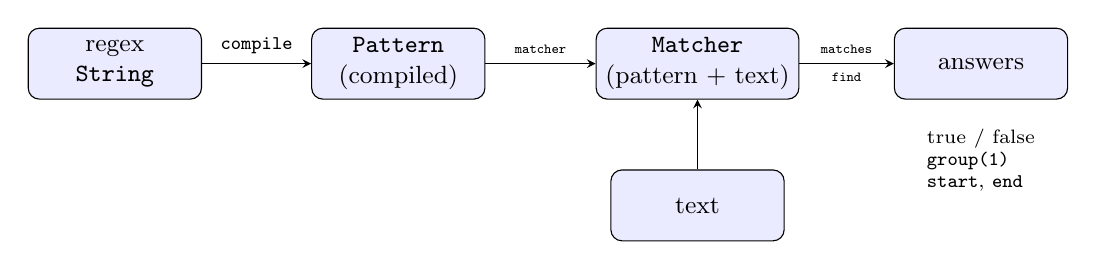
\begin{tikzpicture}[box/.style={draw, rounded corners, fill=blue!8, minimum height=0.9cm, minimum width=2.2cm, align=center, font=\small},
                      >=stealth, every edge/.style={draw, ->}]
    \node[box] (s) at (0,0)    {regex\\\texttt{String}};
    \node[box] (p) at (3.6,0)  {\texttt{Pattern}\\(compiled)};
    \node[box] (m) at (7.4,0)  {\texttt{Matcher}\\(pattern + text)};
    \node[box] (r) at (11,0)   {answers};
    \node[box] (t) at (7.4,-1.8) {text};
    \path (s) edge node[above, font=\scriptsize] {\texttt{compile}} (p)
          (p) edge node[above, font=\tiny] {\texttt{matcher}} (m)
          (t) edge (m)
          (m) edge node[above, font=\tiny] {\texttt{matches}} node[below, font=\tiny] {\texttt{find}} (r);
    \node[font=\scriptsize, align=left, anchor=north] at (11,-0.7) {true / false\\\texttt{group(1)}\\\texttt{start}, \texttt{end}};
  \end{tikzpicture}
  \end{center}
  \begin{itemize}\small
    \item \texttt{Pattern}: the regex turned into a matching program; immutable, safe to share, compile it once.
    \item \texttt{Matcher}: walks one text; remembers where it is (not for sharing between threads).
    \item Shortcuts on \texttt{String}: \texttt{matches}, \texttt{split}, \texttt{replaceAll}, \texttt{replaceFirst}: each compiles the regex again.
  \end{itemize}
\end{frame}
% ~~~~~~~~~~~~~~~~~~~~~~~~~~~~~~~~~~~~~~ A frm




% ~~~~~~~~~~~~~~~~~~~~~~~~~~~~~~~~~~~~~~ V frm
\begin{frame}[t,fragile] \frametitle{Two languages in one line}
  \begin{columns}[T]
    \begin{column}{0.5\textwidth}
      \begin{center}
      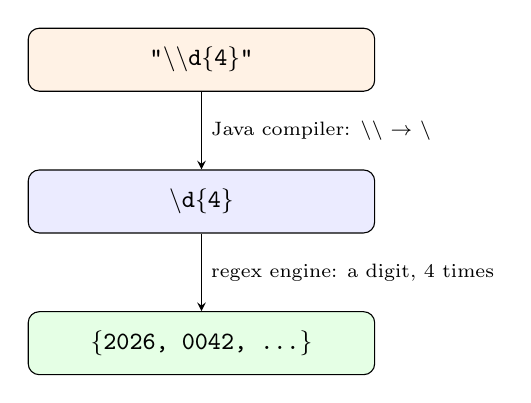
\begin{tikzpicture}[box/.style={draw, rounded corners, minimum width=4.4cm, minimum height=0.8cm, font=\ttfamily\small}, >=stealth]
        \node[box, fill=orange!10] (j) at (0,0)    {"\textbackslash\textbackslash d\{4\}"};
        \node[box, fill=blue!8]    (r) at (0,-1.8) {\textbackslash d\{4\}};
        \node[box, fill=green!10]  (s) at (0,-3.6) {\{2026, 0042, \dots\}};
        \draw[->] (j) -- node[right, font=\scriptsize] {Java compiler: \texttt{\textbackslash\textbackslash} $\to$ \texttt{\textbackslash}} (r);
        \draw[->] (r) -- node[right, font=\scriptsize] {regex engine: a digit, 4 times} (s);
      \end{tikzpicture}
      \end{center}
    \end{column}
    \begin{column}{0.46\textwidth}
      \begin{itemize}\small
        \item In Java source, the regex is inside a string literal.
        \item The compiler reads \texttt{\textbackslash\textbackslash} as one backslash; the regex engine then sees \texttt{\textbackslash d}.
        \item A literal dot: regex \texttt{\textbackslash .}, Java \texttt{"\textbackslash\textbackslash ."}. A literal backslash: regex \texttt{\textbackslash\textbackslash}, Java \texttt{"\textbackslash\textbackslash\textbackslash\textbackslash"}.
        \item Text blocks and string literals both need this; IDEs help when pasting.
      \end{itemize}
    \end{column}
  \end{columns}
\end{frame}
% ~~~~~~~~~~~~~~~~~~~~~~~~~~~~~~~~~~~~~~ A frm




% ~~~~~~~~~~~~~~~~~~~~~~~~~~~~~~~~~~~~~~ V frm
\begin{frame}[t,fragile] \frametitle{One real program}
  \lstcoderightstep[0.6][basicstyle=\ttfamily\scriptsize][basicstyle=\ttfamily\scriptsize]{codeoutput/First.java}{Java}{codeoutput/First.txt}

  \vspace{0.2em}
  \small A date of the form \texttt{yyyy-mm-dd}. \texttt{matches}: the whole text; \texttt{replaceAll}: every place. The form is checked, not the value: \texttt{2026-13-45} matches too.
\end{frame}
% ~~~~~~~~~~~~~~~~~~~~~~~~~~~~~~~~~~~~~~ A frm

% ~~~~~~~~~~~~~~~~~~~~~~~~~~~~~~~~~~~~~~ V
\hSection[Engines]{How Matching Works}
% ~~~~~~~~~~~~~~~~~~~~~~~~~~~~~~~~~~~~~~ A




% ~~~~~~~~~~~~~~~~~~~~~~~~~~~~~~~~~~~~~~ V frm
\begin{frame}[t,fragile] \frametitle{Idea 1: a finite automaton}
  \begin{columns}[T]
    \begin{column}{0.54\textwidth}
      \begin{center}
      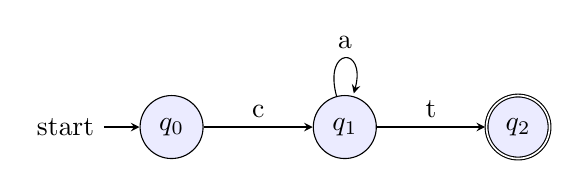
\begin{tikzpicture}[>=stealth, node distance=2.2cm, auto, every state/.style={minimum size=0.8cm, fill=blue!8}]
        \node[state, initial]   (q0)               {$q_{0}$};
        \node[state]            (q1) [right of=q0] {$q_{1}$};
        \node[state, accepting] (q2) [right of=q1] {$q_{2}$};
        \path[->] (q0) edge node {c} (q1)
                  (q1) edge [loop above] node {a} (q1)
                       edge node {t} (q2);
      \end{tikzpicture}
      \end{center}
      \small An automaton for \texttt{ca*t}: \texttt{ct}, \texttt{cat}, \texttt{caaat} end in $q_{2}$; \texttt{ca} stops in $q_{1}$, \texttt{cut} has no arrow for \texttt{u}.
    \end{column}
    \begin{column}{0.42\textwidth}
      \begin{itemize}\small
        \item Every regex (without the extras) can be turned into a machine with finitely many \emph{states}.
        \item Read the text one character at a time and follow the arrow.
        \item At the end: in an accepting (double) state $\Rightarrow$ match.
        \item Time grows only linearly with the text.
      \end{itemize}
    \end{column}
  \end{columns}
\end{frame}
% ~~~~~~~~~~~~~~~~~~~~~~~~~~~~~~~~~~~~~~ A frm




% ~~~~~~~~~~~~~~~~~~~~~~~~~~~~~~~~~~~~~~ V frm
\begin{frame}[t,fragile] \frametitle{Idea 2: try, and go back (backtracking)}
  \begin{columns}[T]
    \begin{column}{0.54\textwidth}


% +++++++++++++++++++++++++++++++++++++++ V alg
%: -Alg. 
\begin{algorithm}[H]
  \caption{Matching by trying}
  \KwIn{a regex as a list of parts $p_{1} \dots p_{k}$, a text $s$}
  \KwOut{true if $s$ matches}
  start with part $p_{1}$ at position 1\;
  \While{a part is left}{
    \eIf{the part can take a (new) choice here}{
      take it, move on to the next part\;
    }{
      go back to the last part that had another choice\;
      \lIf{there is none}{\Return{false}}
    }
  }
  \Return{true if the whole text is used}
\end{algorithm}
% +++++++++++++++++++++++++++++++++++++++ A alg

    \end{column}
    \begin{column}{0.42\textwidth}
      \begin{itemize}\small
        \item Java, Python, JavaScript, Perl work this way.
        \item It allows extras: back-references \texttt{\textbackslash 1}, look-ahead.
        \item \texttt{a*} first takes as many as it can (\emph{greedy}), then gives back one at a time.
        \item Too many choices to go back to: the time can explode (senior level).
      \end{itemize}
    \end{column}
  \end{columns}
\end{frame}
% ~~~~~~~~~~~~~~~~~~~~~~~~~~~~~~~~~~~~~~ A frm




% ~~~~~~~~~~~~~~~~~~~~~~~~~~~~~~~~~~~~~~ V frm
\begin{frame}[t,fragile] \frametitle{Greedy, lazy and the cost of choices}
  \begin{itemize}\small
    \item Text \texttt{<b>Bold</b> and <b>more</b>}, regex \texttt{<b>.*</b>}:
      \texttt{.*} takes everything, gives back until \texttt{</b>} fits: the match runs to the \emph{last} \texttt{</b>}.
    \item Lazy \texttt{<b>.*?</b>}: takes as little as possible: \texttt{<b>Bold</b>}.
    \item Exact \texttt{<b>[\textasciicircum <]*</b>}: only one way to match, so nothing to try again.
    \item With $n$ characters and two ways to split each, a backtracking engine may try up to
  \end{itemize}
  \[
  	2^{n} \ \mathrm{paths}, \qquad 2^{30} \approx 10^{9}
  \]
  \begin{itemize}\small
    \item Good patterns leave few choices: say exactly what may appear.
  \end{itemize}
\end{frame}
% ~~~~~~~~~~~~~~~~~~~~~~~~~~~~~~~~~~~~~~ A frm

% ~~~~~~~~~~~~~~~~~~~~~~~~~~~~~~~~~~~~~~ V
\hSection[Tools]{Regexes Outside Java}
% ~~~~~~~~~~~~~~~~~~~~~~~~~~~~~~~~~~~~~~ A




% ~~~~~~~~~~~~~~~~~~~~~~~~~~~~~~~~~~~~~~ V frm
\begin{frame}[t,fragile] \frametitle{The same idea in a terminal: \texttt{grep}}
  \lstterminal[basicstyle=\ttfamily\tiny]{codeoutput/Grep.txt}

  \vspace{0.1em}
  \small
  \texttt{-E}: extended regex, \texttt{-o}: only the matching part, \texttt{-v}: lines that do \emph{not} match. Run on Linux; macOS Terminal has \texttt{grep} with the same options.
\end{frame}
% ~~~~~~~~~~~~~~~~~~~~~~~~~~~~~~~~~~~~~~ A frm




% ~~~~~~~~~~~~~~~~~~~~~~~~~~~~~~~~~~~~~~ V frm
\begin{frame}[t,fragile] \frametitle{Windows and macOS}
  \begin{itemize}\small
    \item \win: Command Prompt has \texttt{findstr /R} (a very small regex language), PowerShell has \texttt{Select-String} (.NET regex, close to Java). Not run here.
    \item \mac: \texttt{grep -E} in Terminal (as on the previous slide).
    \item Both: IDEs (Eclipse, IntelliJ, VS Code) search and replace with regexes.
  \end{itemize}
  \begin{columns}[T]
    \begin{column}{0.48\textwidth}
      \begin{block}{Windows (not run here)}


% +++++++++++++++++++++++++++++++++++++++ V lst
%: -Lst.
\begin{lstlisting}[style=codesnippet, language={}, basicstyle=\ttfamily\scriptsize]
findstr /R "^[A-Z]" students.txt
powershell -Command "Select-String '[0-9]{11}' students.txt"
\end{lstlisting}
% +++++++++++++++++++++++++++++++++++++++ A lst


      \end{block}
    \end{column}
    \begin{column}{0.48\textwidth}
      \begin{block}{macOS (Terminal)}


% +++++++++++++++++++++++++++++++++++++++ V lst
%: -Lst.
\begin{lstlisting}[style=codesnippet, language=bash, basicstyle=\ttfamily\scriptsize]
grep -E '^[A-Z]' students.txt
grep -E -o '[0-9]{11}' students.txt
\end{lstlisting}
% +++++++++++++++++++++++++++++++++++++++ A lst


      \end{block}
    \end{column}
  \end{columns}
\end{frame}
% ~~~~~~~~~~~~~~~~~~~~~~~~~~~~~~~~~~~~~~ A frm

% ~~~~~~~~~~~~~~~~~~~~~~~~~~~~~~~~~~~~~~ V
\hSection[Limits]{Limits}
% ~~~~~~~~~~~~~~~~~~~~~~~~~~~~~~~~~~~~~~ A




% ~~~~~~~~~~~~~~~~~~~~~~~~~~~~~~~~~~~~~~ V frm
\begin{frame}[t,fragile] \frametitle{What a regex cannot (or should not) do}
  \begin{itemize}\small
    \item \textbf{Counting without a bound}: ``as many \texttt{(} as \texttt{)}'' is not regular; brackets, HTML, JSON need a parser.
    \item \textbf{Meaning}: \texttt{\textbackslash d\{2\}\textbackslash .\textbackslash d\{2\}\textbackslash .\textbackslash d\{4\}} accepts \texttt{31.02.2026}; the calendar check needs code (\texttt{LocalDate.parse}).
    \item \textbf{Readability}: \texttt{\textasciicircum (?=.*\textbackslash d)(?=.*[a-z]).\{8,\}\$} is hard to read; comment it, name the groups, test it.
    \item \textbf{Speed}: some patterns take exponential time on unlucky input.
    \item \textbf{Security}: a pattern built from user input can do unwanted things.
  \end{itemize}
  \vspace{0.5em}
  \hRemark{A regex is a tool for the \emph{form} of text, not for its structure or meaning.}
\end{frame}
% ~~~~~~~~~~~~~~~~~~~~~~~~~~~~~~~~~~~~~~ A frm

% ~~~~~~~~~~~~~~~~~~~~~~~~~~~~~~~~~~~~~~ V
\hSection[Levels]{The Road Ahead}
% ~~~~~~~~~~~~~~~~~~~~~~~~~~~~~~~~~~~~~~ A




% ~~~~~~~~~~~~~~~~~~~~~~~~~~~~~~~~~~~~~~ V frm
\begin{frame}[t,fragile] \frametitle{What each level adds}
  \begin{center}\small
  \begin{tabular}{@{}lL{0.7\textwidth}@{}}
    \toprule
    \textbf{level}  & \textbf{topics} \\
    \midrule
    freshman        & \texttt{matches}, classes, quantifiers, \texttt{split}, \texttt{replaceAll}, escaping, error messages \\
    sophomore       & \texttt{Pattern}/\texttt{Matcher}, \texttt{find}, groups, flags, look-ahead, greedy and lazy, unit tests \\
    junior          & Unicode and Turkish letters, back-references, look-around, possessive, newer APIs, speed \\
    senior          & automata, engines, ReDoS, stack overflow, time limits, RE2/J, regex injection \\
    examples        & every concept of this deck as a real program \\
    \bottomrule
  \end{tabular}
  \end{center}
\end{frame}
% ~~~~~~~~~~~~~~~~~~~~~~~~~~~~~~~~~~~~~~ A frm

% ~~~~~~~~~~~~~~~~~~~~~~~~~~~~~~~~~~~~~~ V
\hSection[Summary]{Summary}
% ~~~~~~~~~~~~~~~~~~~~~~~~~~~~~~~~~~~~~~ A




% ~~~~~~~~~~~~~~~~~~~~~~~~~~~~~~~~~~~~~~ V frm
\begin{frame}[t,fragile] \frametitle{Summary}
  \begin{itemize}\small
    \item A regex describes a set of strings; a text matches if it is in the set.
    \item Building blocks: literals, classes, quantifiers, anchors, groups, alternation.
    \item In Java: compile to a \texttt{Pattern}, ask a \texttt{Matcher}; write every \texttt{\textbackslash} twice in source.
    \item Engines: an automaton (linear, fewer features) or backtracking (more features, can be slow).
    \item Regexes check the form of text; use parsers and code for structure and meaning.
  \end{itemize}
\end{frame}
% ~~~~~~~~~~~~~~~~~~~~~~~~~~~~~~~~~~~~~~ A frm




% ~~~~~~~~~~~~~~~~~~~~~~~~~~~~~~~~~~~~~~ V frm
\begin{frame}[t,fragile] \frametitle{Exercises}
  \begin{enumerate}\small
    \item Give three strings that match and three that do not: \texttt{[A-Z][a-z]+}, \texttt{\textbackslash d+(\textbackslash .\textbackslash d\{2\})?}, \texttt{(ab|ba)*}.
    \item Write a regex for: a Yeditepe course code (\texttt{CSE101}), a time (\texttt{09:30}), a plate number (\texttt{34 ABC 123}).
    \item Draw an automaton for \texttt{(ab)*} and for \texttt{a(b|c)d}.
    \item Write the Java string literal for the regexes \texttt{\textbackslash d+\textbackslash .\textbackslash d+} and \texttt{C:\textbackslash\textbackslash Users}.
    \item Why does \texttt{find} with \texttt{\textasciicircum cat|dog\$} succeed on \texttt{catalog} and \texttt{hotdog}? Fix it.
  \end{enumerate}
\end{frame}
% ~~~~~~~~~~~~~~~~~~~~~~~~~~~~~~~~~~~~~~ A frm




% ~~~~~~~~~~~~~~~~~~~~~~~~~~~~~~~~~~~~~~ V frm
\begin{frame}[t,fragile]
	\begin{center}
		\vspace{4cm}
		\hRemark{\Huge Questions?}
	\end{center}
\end{frame}
% ~~~~~~~~~~~~~~~~~~~~~~~~~~~~~~~~~~~~~~ A frm



\end{document}
